% case 3 results

\section{Case overview}

Case Three is about a global collaboration aiming to revolutionise bee research. Many food crops rely on honey bees for pollination. For reasons not yet understood, bee colonies around the world are collapsing at an alarming rate. Unchecked, this may lead to rising food shortages and possibly widespread famine. Research into colony collapse disorder has tended to be piecemeal without a sense of urgency. One major research objective is to gain a deeper understanding of environmental factors that influence bee movement in and out of hives. \medskip

National Research Laboratories is developing miniaturised sensor technology that can be carried by insects. Their long-term research goal is to use nanotechnology, powered by high-frequency wing movement, to tap into the extraordinary sensing capability of insects. Achieving this goal will take several years. However, as part of their research, National Research Laboratories have developed a novel approach for tracking bee movements. This involves attaching miniaturised electronic tags to bees. Sensors register when bees leave and return to the hive. Bee movements are transmitted in near real-time to a central data repository. By massively scaling data collection efforts worldwide, it should be possible to isolate interesting patterns of bee movement using sophisticated computer algorithms developed for big data analysis.\medskip

Finding correlations between patterns of bee movement with other environmental information e.g. local climate variables, traces of pesticides, co-occurrence of bee predators, or presence of parasites, should shed new light on what is driving colony collapse disorder. This requires worldwide coordination of bee research efforts. National Research Laboratories has invited technology providers and bee researchers from across the world to work together to make this happen. Various technology providers and research institutions have agreed to work together to help coordinate data collection efforts. National Research Laboratories has been supplying sensor kits to bee researchers to enable them to collect and communicate data to the central data repository. Getting these to work reliably is largely dependent on the absorptive capacity and enthusiasm of each partner. Many bee researchers consider the use of advanced sensor technology and big data analysis quite revolutionary and exciting. Others have yet to be convinced this approach will deliver meaningful information but are willing to give it a fair go. National Research Laboratories has received much publicity around the formation of a global collaboration for coordinated honey bee research, which has resulted in feelings of resentment among some bee researchers. Who ultimately should be driving this initiative within National Research Laboratories also remains a contentious issue. All this creates an interesting dynamic around knowledge sharing and idea generation. \medskip

The global collaboration for coordinated honey bee research is still in its infancy. New partners are coming aboard as the collaboration gains traction. What sets this case apart from the others is the lack of a strong commercial focus. Each partner is pursuing their own bee research agenda independently of others. Knowledge sharing is limited to issues surrounding the deployment and operation of the sensor technology. How best to exploit the massive amounts of data being collected from across the world is not receiving much attention yet.\medskip  

This case examines knowledge sharing behaviour between 40 people from 16 organisations in 6 different countries involved in the collaboration. Many of the people work for National Research Laboratories. Partner organisations have between one and four representatives actively involved in the collaboration. Three partners are technology providers, the rest are either bee keepers or bee researchers from other agencies. Case Three involves network, structure, process, and customer engagement innovation (Figure \ref{fig:innovation_type}).


\section{Quantitative analysis}

\subsection{Descriptive statistics}

Of the 45 people invited to participate in this case study, 40 agreed to take part (89\% response rate). The people who declined to participate expressed strong negative sentiments towards the collaboration.

\subsubsection{Demographics}

Of the 40 people who did agree to participate, seven identified as female, the rest as male. The age of participants ranges from 24 to 66 years (average age = 44.8 years, median age = 44 years). Relevant work experience ranged from 1 to 40 years (average experience = 13.9 years, median experience = 11.5 years). Current job tenure ranged from 1 to 33 years (average tenure = 9.1 years, median tenure = 4.5 years). Box-plots showing the distribution of age, work experience and tenure of participants in each case study are presented in Figure \ref{fig:ageexperience}.\medskip

Figure \ref{fig:edlevelrose} shows how education levels differ in each case study. Participants in this case study have education levels ranging from secondary level to doctoral level. A huge majority of participants have a doctoral degree. This case is also dominated by people with an educational background in either agriculture or natural and physical sciences. Less represented educational backgrounds include engineering, information technology, management, architecture, and society and culture (Figure \ref{fig:edfieldrose}).

\subsubsection{Basic network statistics}

Descriptive statistics for the explicit and tacit knowledge provider networks and idea contributor network are presented in Table \ref{ds_c3}. All the networks share a common set of nodes (40 in total). Because some people declined to participate in this case study, there are missing nodes in the data set (nodes 5, 6, 30, 31, and 37). Compared to the other case studies, the networks in this case are fairly sparse (density ranging from 0.06 to 0.08). This is not surprising, given the immaturity of this particular collaboration. The idea contributor network has more than twice the number of reciprocated ties than what the explicit and tacit knowledge provider networks have, suggesting a broad preference for creative interaction over knowledge sharing.\medskip

\begin{table}[]
	\small
	\centering
	\caption{Descriptive network statistics - Case 3}
	\label{ds_c3}
	\begin{tabular}{@{}lcccccc@{}}
		\toprule
		& \multicolumn{1}{l}{} & \multicolumn{1}{l}{} & \multicolumn{1}{l}{} & \multicolumn{3}{c}{Dyad Census}	\\ \cline{5-7}
		Network						& Nodes			& Arcs			& Density	& Mutual		& Asymmetric	& Null		\\ \midrule
		Explicit Knowledge Provider & 40			& 121			& 0.08		& 11			& 99			& 670		\\
		Tacit Knowledge Provider    & 40			& 93			& 0.06		& 14			& 65			& 701		\\
		Idea Contributor            & 40			& 132			& 0.08		& 29			& 74			& 677		\\ \bottomrule
	\end{tabular}
\end{table}

Network diagrams for the explicit and tacit knowledge provider networks and idea contributor network are presented in Figure \ref{fig:thesisnetworkscase3}. Arrows indicate the direction of knowledge and idea flows. Nodes are sized according to Burt's constraint measure and colour-coded by employer affiliation. The network diagrams indicate the collaboration is dominated by one highly central individual(node 10) who also works for the dominant organisation in this collaboration. Employees from this organisation have the greatest access to knowledge and ideas within the collaboration. This is not the case for employees in other organisations, who judging by node size, are quite constrained in terms of access to network resources.\medskip

\begin{landscape}
\begin{figure}
	\centering
	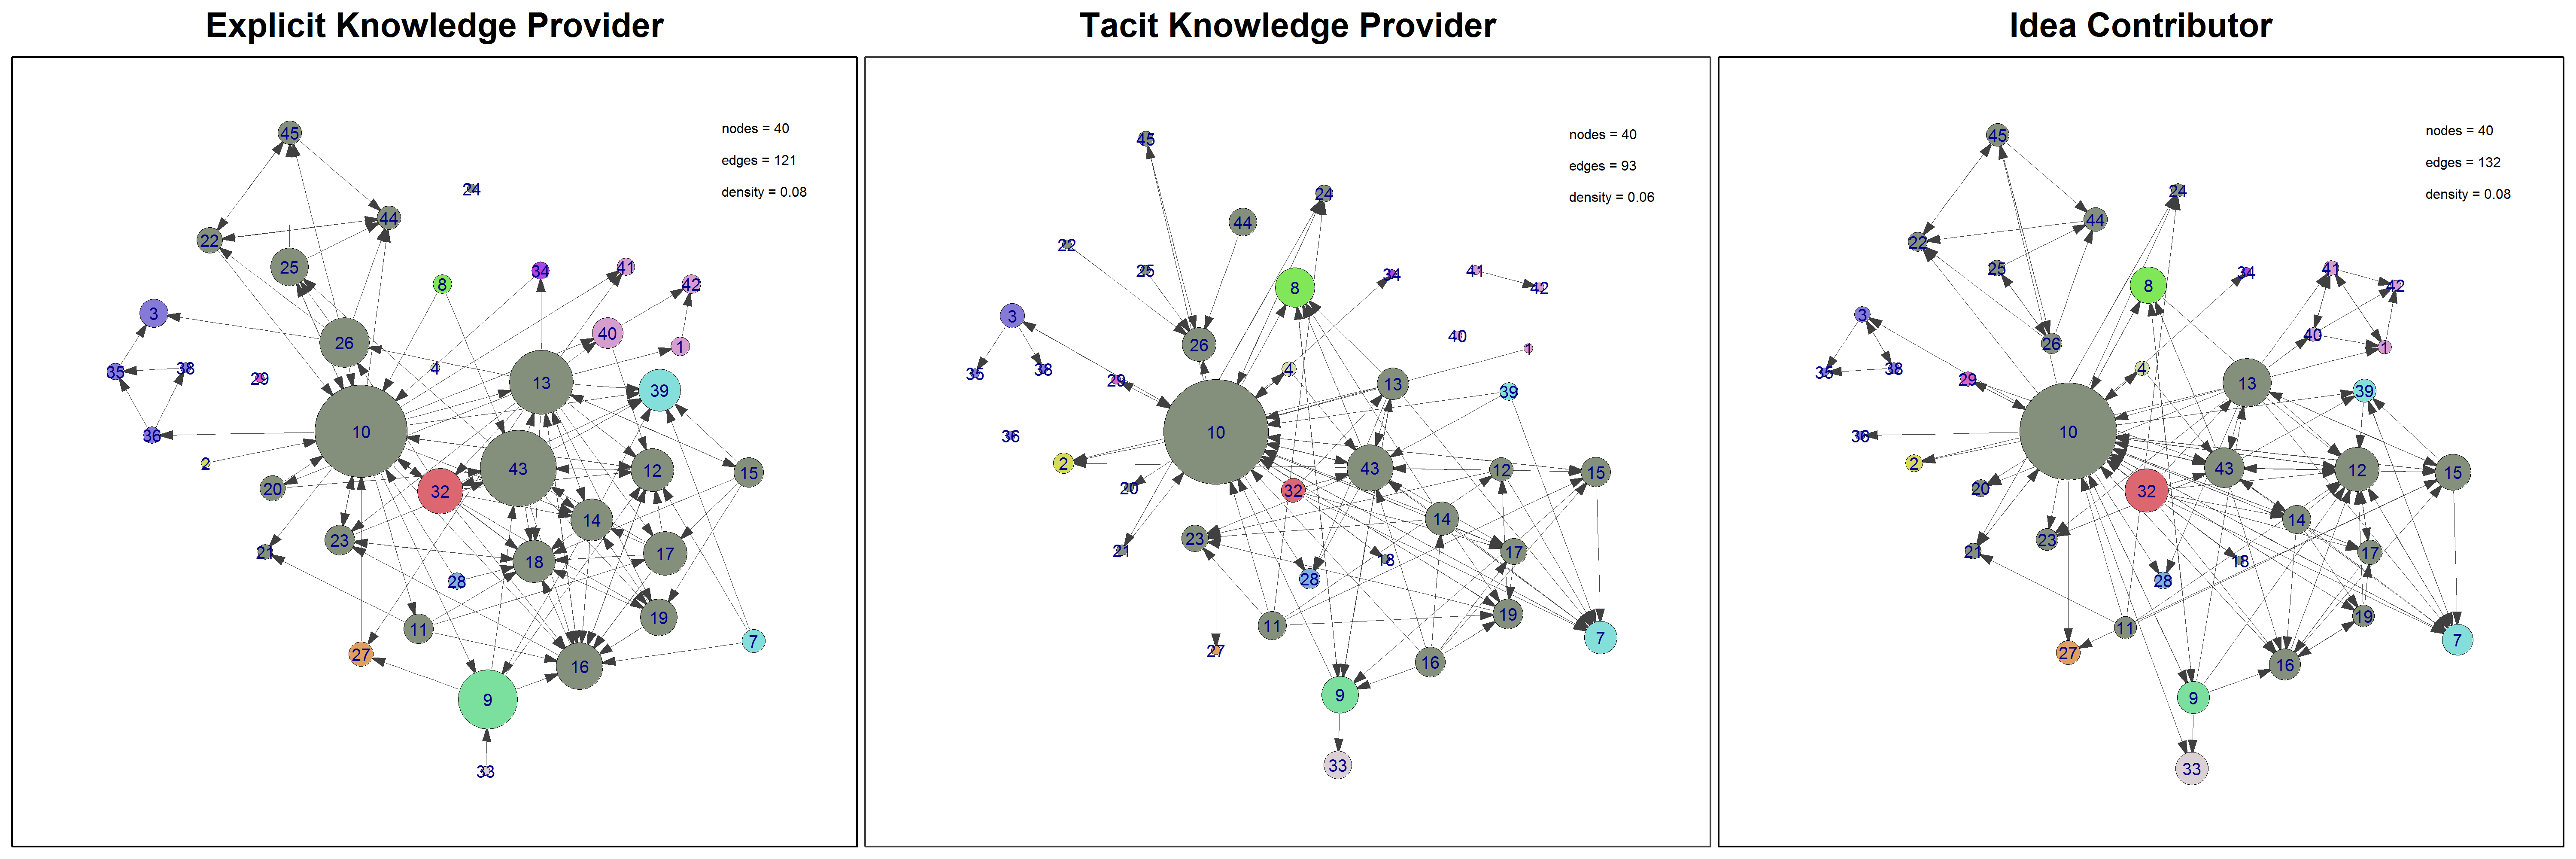
\includegraphics[width=1.0\linewidth]{Images/thesis_networks_case3}
	\caption{Network diagrams - Case 3}
	\label{fig:thesisnetworkscase3}
\end{figure}
\end{landscape}

Case 3 is a global initiative with participants based in several different countries. Figure \ref{fig:sphdistancecase3} depicts the physical separation between nodes measured in kilometres (calculated using work-place postcodes as a geographic reference). There are a few small clusters of co-located nodes but for the most part, participants in this collaboration are fairly distant from each other. This may explain why knowledge being shared is mostly explicit in nature.  \medskip  

\begin{figure}
	\centering
	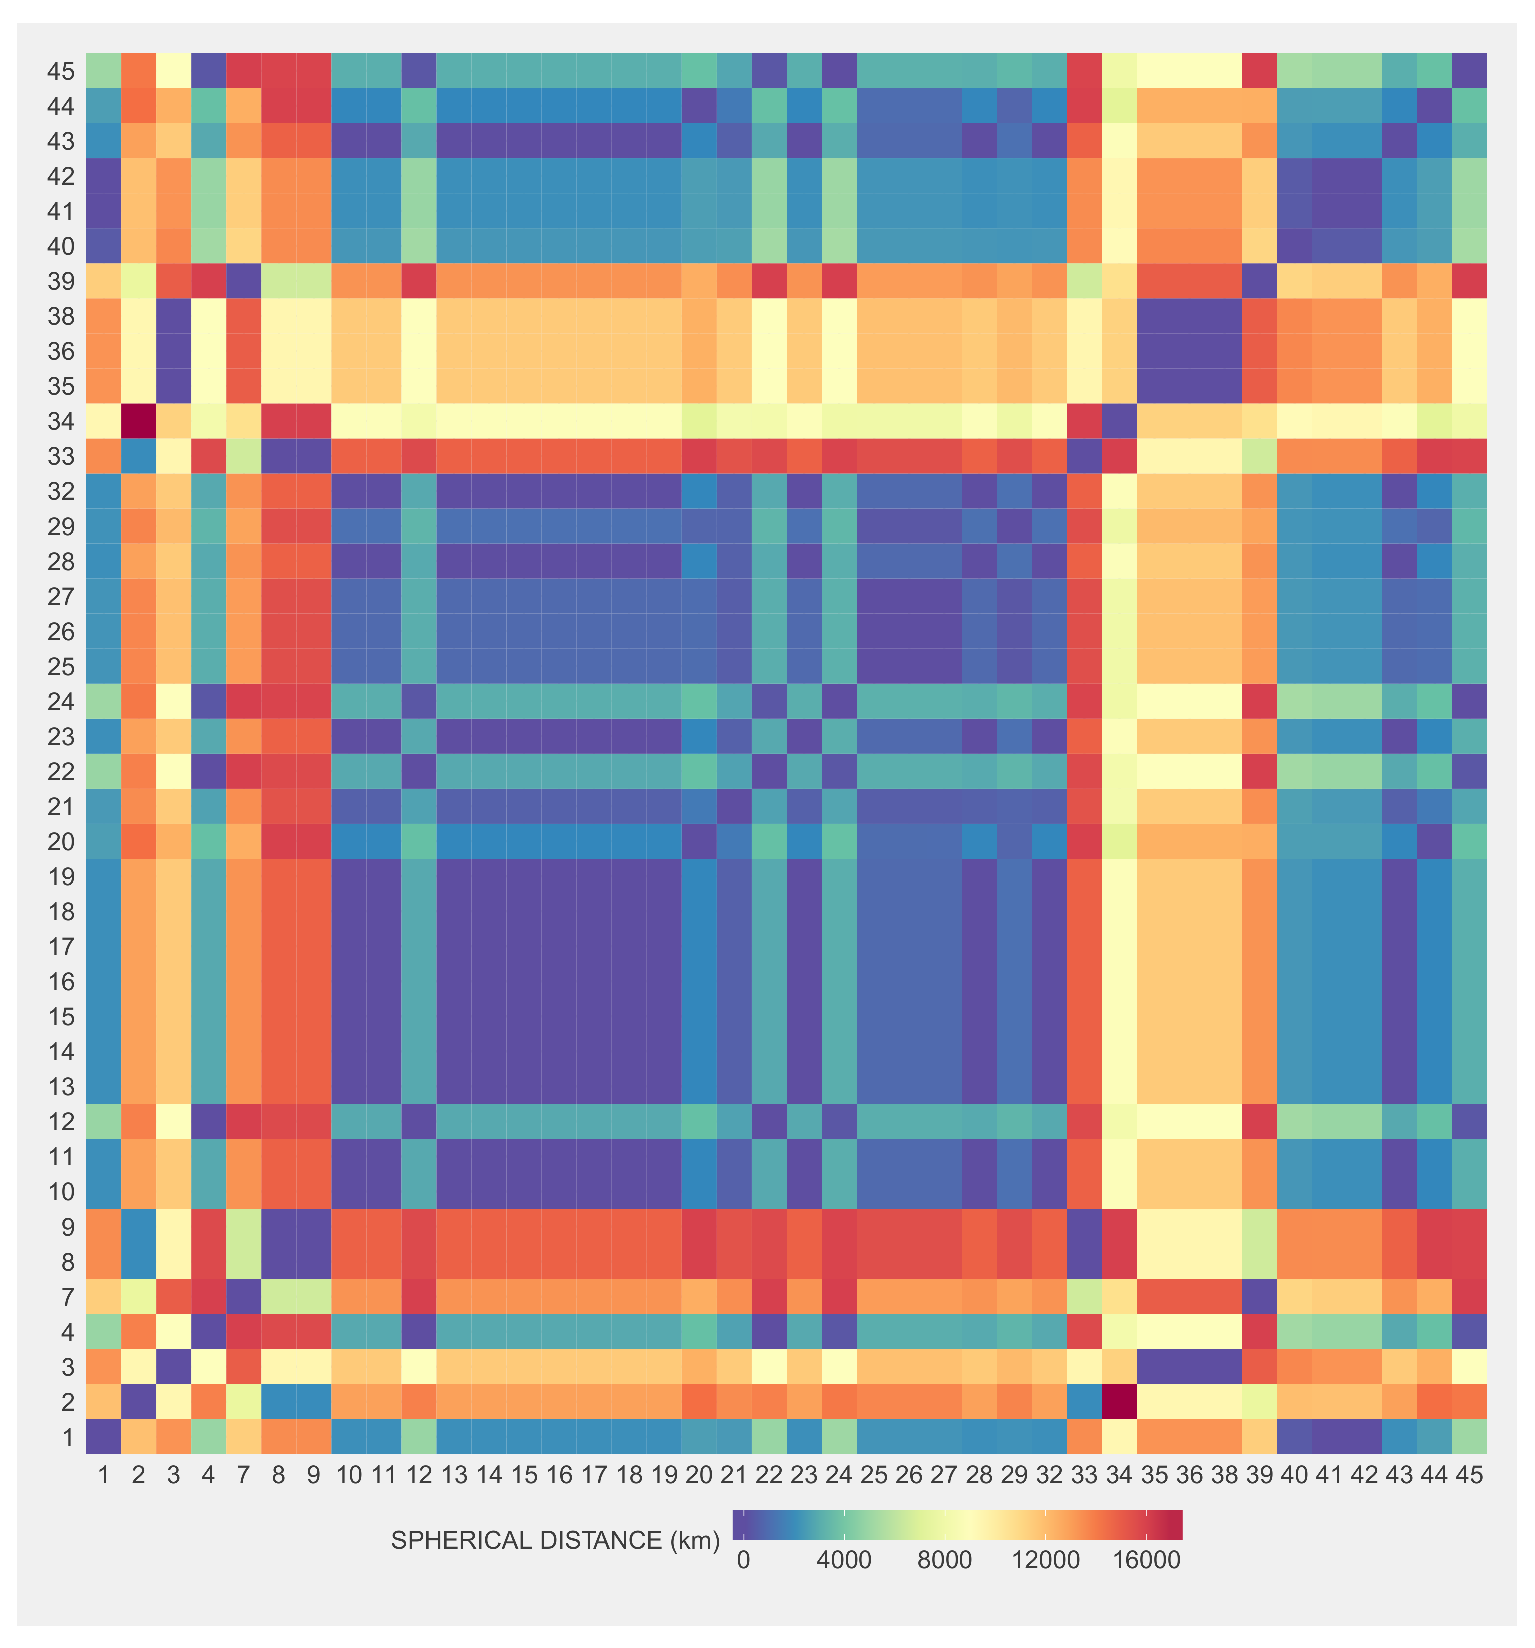
\includegraphics[width=0.7\linewidth]{Images/sph_distance_case3}
	\caption{Distance between nodes - Case 3}
	\label{fig:sphdistancecase3}
	\end{figure}


\subsubsection{Two-path brokerage statistics}

Brokerage roles in Case 3 are quite different to those observed in Cases 1 and 2. Figure \ref{fig:gfbrokeragecase3} shows very little itinerant brokerage in the explicit and tacit knowledge provider networks and idea contributor network. While there appears to be much knowledge and idea exchange between partner organisations, the high level of coordination brokerage suggests much of the innovative activity in Case 3 is internally focused. This may have something to do with the physical separation between participants in this collaboration.\medskip 


\begin{figure}
	\centering
	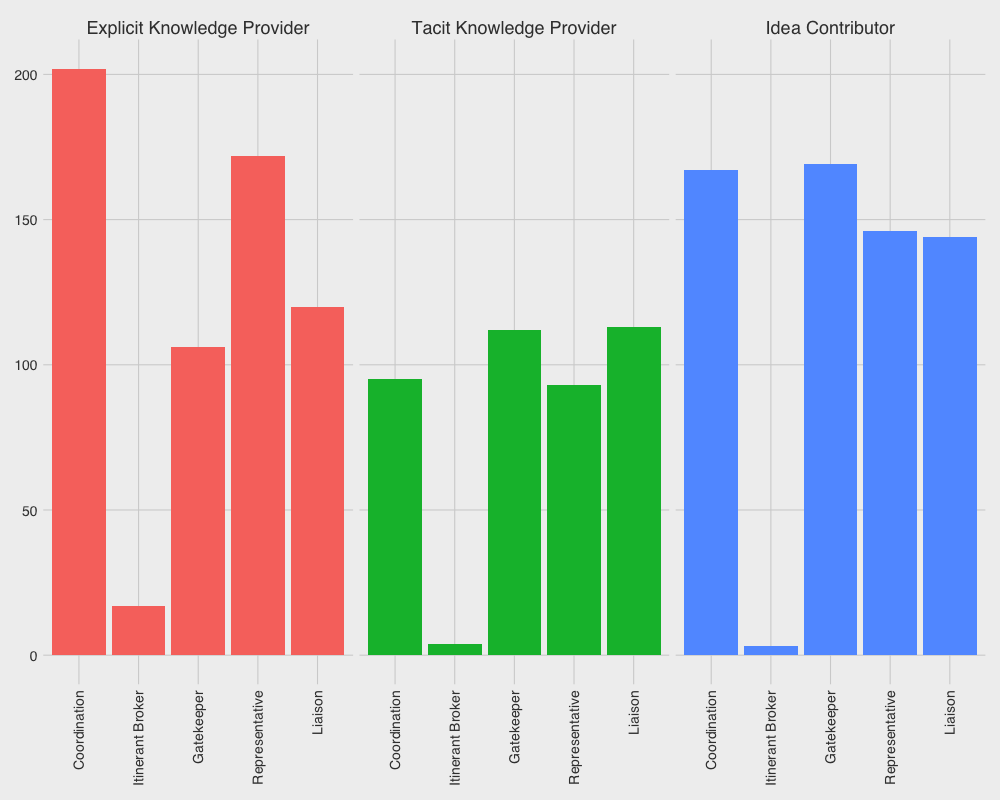
\includegraphics[width=0.7\linewidth]{Images/gf_brokerage_case3}
	\caption{Gould-Fernandez brokerage roles by employer affiliation - Case 3}
	\label{fig:gfbrokeragecase3}
\end{figure}





\subsection{Exponential random graph modelling}

\subsubsection{Autonomous motivation as a predictor of knowledge sharing}

Table \ref{c3_q1} contains the parameter estimates with standard errors in brackets for Model I (explicit knowledge provider) and Model J (tacit knowledge provider). The estimation procedure successfully converged for all the modelled parameters. Goodness of fit statistics for each model were less than 1 in absolute value for almost all the features not explicitly modelled, indicating these fit the data reasonably well. Results are again broken down according to purely structural effects, actor-relation effects, and network covariate effects. \medskip

Referring to the purely structural effects, there is a significant and positive effect for path closure and multiple connectivity in the explicit knowledge provider network. Path closure indicates a tendency for structural holes to close i.e. evidence that explicit knowledge is being socialised. The significant positive effect for multiple connectivity points to brokerage being a key feature of explicit knowledge exchange. The tacit knowledge provider network also has a significant and positive effect for path closure. Like explicit knowledge, there is a tendency for tacit knowledge to be socialised. However, the significant and negative effect for cyclic closure in the tacit knowledge provider network suggests tacit knowledge is socialised very selectively. The significant and positive effect for activity spread in the tacit knowledge provider network indicates some actors are sending significantly more tacit knowledge than others.\medskip

In terms of actor-relation effects, the explicit knowledge provider network has a significant and positive homophily effect for employer match. This indicates a tendency for individuals to share explicit knowledge with fellow employees, rather than with people in other organisations. We see a significant negative receiver effect for self-efficacy and employer mismatch reciprocity in the tacit knowledge provider network. Individuals with high self-efficacy are less likely to receive tacit knowledge. This suggests people with higher levels of self-efficacy may be less inclined to seek out tacit knowledge. The negative effect for employer mismatch reciprocity indicates there is little reciprocal exchange of tacit knowledge across organisational boundaries. There is a significant positive receiver effect for autonomous motivation in the tacit knowledge provider network, indicating autonomously motivated individuals are more likely to seek out and acquire tacit knowledge. However, the significant and positive homophily effect for broad education field in the tacit knowledge provider network suggests individuals are more likely to seek tacit knowledge from people in the same field as them. The significant and positive effect for employer mismatch reciprocity in the tacit knowledge provider network indicates the sharing of tacit knowledge between organisations is reciprocal in nature. \medskip

With respect to network covariate effects, hierarchy has a strong and positive effect in both the explicit and tacit knowledge provider networks indicating individuals are more likely to share knowledge with those they report to in the collaboration. Spatial proximity has a significant and negative effect in both the explicit and tacit knowledge provider networks. This suggests a tendency to only share knowledge with people in close proximity.\medskip

The modelling tells us is that autonomous motivation has no significant effect on explicit knowledge sharing but does have a significant receiver effect on tacit knowledge sharing. There is a general tendency to socialise both explicit and tacit knowledge. However, employer mismatch reciprocity in the tacit knowledge provider network indicates much of the collaboration is done through tacit knowledge sharing.\medskip


\begin{table}[]
	\centering
	\caption{Autonomous motivation as an antecedent for knowledge sharing - Case 3}
	\label{c3_q1}
	\begin{threeparttable}
		\begin{tabular}{@{}lrlrl@{}}
			\toprule
			& \multicolumn{4}{@{}c@{}}{Estimate (SE)} \\ \cline{2-5}
			& \multicolumn{2}{@{}c@{}}{\begin{tabular}[c]{@{}c@{}}Explicit\\ Knowledge\end{tabular}} & \multicolumn{2}{@{}c@{}}{\begin{tabular}[c]{@{}c@{}}Tacit\\ Knowledge\end{tabular}} \\ \midrule
			\textbf{Purely structural effects (endogenous)} &         	&          	&       	&         	\\
			Arc (edge)       								& -3.959  	& (1.756)* 	& -8.068	& (1.781)*	\\
			Reciprocity (mutuality)                         & -0.634  	& (0.511)  	& 0.488 	& (0.750) 	\\
			TwoPath (simple connectivity)                   & -0.204  	& (0.131)  	& -0.082	& (0.133) 	\\
			AinS (popularity spread)                        & 0.454   	& (0.286)  	& 0.318 	& (0.315) 	\\
			AoutS (activity spread)                         & 0.504   	& (0.301)  	& 0.809 	& (0.299)*	\\
			AT-T (path closure)                             & 0.546   	& (0.256)* 	& 0.735 	& (0.245)*	\\
			AT-C (cyclic closure)                           & -0.043  	& (0.135)  	& -0.607	& (0.182)*	\\
			A2P-T (multiple connectivity)                   & 0.315   	& (0.139)* 	& 0.203 	& (0.128) 	\\
															&         	&          	&       	&         	\\
			\textbf{Actor-relation effects (exogenous)}     &         	&          	&       	&         	\\
			age (difference) 								& -0.023  	& (0.014)  	& -0.010	& (0.014) 	\\
			work.experience (sender)                        & -0.002  	& (0.012)  	& -0.004	& (0.012) 	\\
			work.experience (receiver)                      & -0.008  	& (0.012)  	& 0.024 	& (0.013) 	\\
			education.level (sender)                        & 0.119   	& (0.141)  	& 0.134 	& (0.141) 	\\
			education.level (receiver)                      & -0.018  	& (0.111)  	& 0.079 	& (0.116) 	\\
			personality.openness (sender)                   & -0.323  	& (0.595)  	& 0.074 	& (0.516) 	\\
			personality.openness (receiver)                 & 0.558   	& (0.569)  	& -0.493	& (0.603) 	\\
			self.efficacy (sender)                          & 0.341   	& (0.987)  	& 0.752 	& (1.042) 	\\
			self.efficacy (receiver)                        & -0.039  	& (0.944)  	& -2.576	& (1.060)* 	\\
			identification.collab (product)                 & -0.683  	& (0.66)   	& -1.278	& (0.824) 	\\
			autonomous.motivation (sender)                  & -0.598  	& (0.633)  	& 0.410 	& (0.745) 	\\
			autonomous.motivation (receiver)                & 0.007   	& (0.662)  	& 3.577 	& (1.091)*	\\
			broad.education.field (match)                   & 0.379   	& (0.242)  	& 0.594 	& (0.261)*	\\
			employer (match) 								& 0.596   	& (0.287)* 	& 0.474 	& (0.319) 	\\
			employer (mismatch reciprocity)                 & -0.351  	& (1.177)  	& 1.968 	& (0.821)*	\\
															&         	&          	&       	&         	\\
			\textbf{Network covariate effects (exogenous)}  &         	&          	&       	&         	\\
			report.to.net (heirarchy)                       & 1.080   	& (0.395)* 	& 1.169 	& (0.448)*	\\
			log.spherical.distance.net (spatial proximity)  & -0.201  	& (0.043)* 	& -0.165	& (0.038)*	\\ \bottomrule
		\end{tabular}
		\begin{tablenotes}
			\small
			\item [*] Significant effect.
		\end{tablenotes}
	\end{threeparttable}
\end{table}


\subsubsection{Role of tacit knowledge in creative interaction}

Table \ref{c3_q3} lists the parameter estimates with standard errors in brackets for the idea contributor network (Model L). The estimation procedure successfully converged for all the modelled parameters. Goodness of fit statistics were under 2 in absolute value for features not explicitly modelled, indicating Model L fits the data well. Results are again broken down according to purely structural effects, actor-relation effects, and network covariate effects.\medskip 

Examining the purely structural effects, there is a significant and positive effect for reciprocity and path closure in the idea contributor network. This implies the sharing of ideas is both reciprocal in nature and socially intensive, pointing to substantial creative interaction. However, the significant and negative effect for cyclic closure suggests individuals tend to be quite selective in their creative interactions. The significant and negative effect for popularity spread suggests relatively few individuals in the collaboration are attracting ideas from multiple others.\medskip

Referring to actor-relation effects, there is a significant and positive receiver effect for both work experience and autonomous motivation, suggesting individuals with more work experience and greater autonomous motivation are more receptive of ideas. There is a significant and positive sender effect for openness to experience, indicating those more open to experience are inclined to contribute ideas. Contrary to expectations is the significant and negative sender effect for self-efficacy. Despite feeling competent at their job, enjoying higher levels of autonomy, and seeing themselves as creative, individuals with higher levels of self-efficacy are less likely to contribute ideas. The significant and negative effect for identification with the collaboration implies individuals still contribute ideas even though they do not identify strongly with the collaboration.\medskip

Considering network covariate effects, there is a significant and positive effect for both explicit and tacit provider networks (also observed in Cases 1 and 2). However, the effect is stronger for the tacit knowledge provider network, suggesting creative interaction is a little more likely to emerge through tacit knowledge sharing than explicit knowledge sharing. The significant and positive effect for hierarchy indicates individuals are more likely to contribute ideas to people they report to in the collaboration.
      

\begin{table}[]
	\centering
	\caption{Tacit knowledge sharing as an antecedent to creative interaction - Case 3}
	\label{c3_q3}
	\begin{threeparttable}
		\begin{tabular}{@{}lrl@{}}
			\toprule
			& \multicolumn{2}{@{}c@{}}{Estimate (SE)} \\ \midrule
			\textbf{Purely structural effects (endogenous)}      &                &                  \\
			Arc (edge)                                           & -8.519         & (2.702)*         \\
			Reciprocity (mutuality)                              & 1.431          & (0.591)*         \\
			TwoPath (simple connectivity)                        & 0.076          & (0.095)          \\
			AinS (popularity spread)                             & -1.563         & (0.454)*         \\
			AoutS (activity spread)                              & -0.350         & (0.377)          \\
			AT-T (path closure)                                  & 1.112          & (0.266)*         \\
			AT-C (cyclic closure)                                & -0.523         & (0.153)*         \\
			A2P-T (multiple connectivity)                        & -0.095         & (0.089)          \\
			&                &                  \\
			\textbf{Actor-relation effects (exogenous)}          &                &                  \\
			age (difference)                                     & 0.028          & (0.019)          \\
			work.experience (sender)                             & 0.007          & (0.017)          \\
			work.experience (receiver)                           & 0.053          & (0.019)*         \\
			education.level (sender)                             & 0.387          & (0.252)          \\
			education.level (receiver)                           & 0.136          & (0.172)          \\
			personality.openness (sender)                        & 1.668          & (0.803)*         \\
			personality.openness (receiver)                      & 0.867          & (0.953)          \\
			self.efficacy (sender)                               & -3.103         & (1.401)*         \\
			self.efficacy (receiver)                             & -2.639         & (1.643)          \\
			identification.collab (product)                      & -2.524         & (1.120)*          \\
			autonomous.motivation (sender)                       & 0.177          & (1.044)          \\
			autonomous.motivation (receiver)                     & 3.847          & (1.322)*         \\
			broad.education.field (match)                        & -0.547         & (0.355)          \\
			employer (match)                                     & 0.260          & (0.417)          \\
			employer (mismatch reciprocity)                      & -0.244         & (0.732)          \\
			&                &                  \\
			\textbf{Network covariate effects (exogenous)}       &                &                  \\
			tacit.knowledge.net (tacit knowledge provider)       & 4.842          & (0.481)*         \\
			explicit.knowledge.net (explicit knowledge provider) & 3.745          & (0.450)*          \\
			report.to.net (hierarchy)                            & 1.873          & (0.572)*         \\
			log.spherical.distance.net (spatial proximity)       & -0.008         & (0.046)          \\ \bottomrule
			\end{tabular}
			\begin{tablenotes}
				\small
				\item [*] Significant effect.
			\end{tablenotes}
	\end{threeparttable}
\end{table}

\section{Qualitative analysis}

\begin{landscape}
	\begin{table}[]
		\centering
		\caption{Case 3 interview participants}
		\label{c3_interviews}
		\begin{threeparttable}
			\begin{tabular}{@{}cccccccccccc@{}}
				\toprule
				Node & Employer & \begin{tabular}[c]{@{}c@{}}Interview \\ Date\end{tabular} & Age & \begin{tabular}[c]{@{}c@{}}Relevant\\ Work \\ Experience\end{tabular} & \begin{tabular}[c]{@{}c@{}}Current \\ Job \\ Tenure\end{tabular} & \begin{tabular}[c]{@{}c@{}}Education\\ Level\end{tabular} & \begin{tabular}[c]{@{}c@{}}Broad\\ Education\\ Field\end{tabular} & \begin{tabular}[c]{@{}c@{}}In-degree\\ Centrality\end{tabular} & \begin{tabular}[c]{@{}c@{}}Out-degree\\ Centrality\end{tabular} & \begin{tabular}[c]{@{}c@{}}Eigenvector\\ Centrality\end{tabular} & \begin{tabular}[c]{@{}c@{}}Burt's\\ Constraint\\ Measure\end{tabular} \\ \midrule
				2    & 2  &   TBA     & 36  & 5                   & 3            & 8       & 5               & 3         & 1          & 0.17                    & 0.43       \\
				7    & 7  &   TBA     & 53  & 22                  & 18           & 8       & 1               & 8         & 5          & 0.38                    & 0.27       \\
				8    & 8  &   TBA     & 37  & 16                  & 3            & 8       & 2               & 8         & 4          & 0.28                    & 0.27       \\
				9    & 9  &   TBA     & 50  & 26                  & 26           & 8       & 5               & 10        & 8          & 0.38                    & 0.21       \\
				10   & 10 &  16/03/16       & 45  & 3                   & 8            & 8       & 1               & 34        & 36         & 1.00                    & 0.09       \\
				13   & 10 &  13/05/16      & 41  & 4                   & 4            & 8       & 1               & 9         & 26         & 0.68                    & 0.17       \\
				16   & 10 &  12/09/16      & 47  & 16                  & 9            & 7       & 2               & 12        & 11         & 0.59                    & 0.21       \\
				22   & 10 &  19/09/16      & 61  & 32                  & 32           & 8       & 5               & 6         & 4          & 0.15                    & 0.37       \\
				39   & 7  &  09/09/16      & 30  & 4                   & 2            & 7       & 1               & 7         & 3          & 0.31                    & 0.30       \\
				41   & 1  &  07/10/16      & 24  & 5                   & 4            & 6       & 1               & 2         & 1          & 0.08                    & 0.35       \\ \bottomrule
			\end{tabular}
			\begin{tablenotes}
				\small
				\item Notes:
				\item 1. Numbers in the education level/broad education field columns are the same as those used in the Australian Standard Classification for Education.
				\item 2. Statistics for the undifferentiated knowledge provider network.
				\item 3. In-degree centrality refers to the number of incoming knowledge ties. Out-degree centrality refers to the number of outgoing knowledge ties.
				\item 4. Eigenvector centrality refers to the relative importance of a node (connectivity with other high degree-centrality nodes) on a scale of 0 to 1.
				\item 5. Burt's constraint measure refers to access to network resources on a scale of 0 to 1. Lower values mean greater access to network resources.
			\end{tablenotes}
		\end{threeparttable}
	\end{table}
\end{landscape}

